\documentclass{article}
%-------------------------------------------------------------------
% Paquetes necesarios
\usepackage[utf8]{inputenc} % Para caracteres especiales
\usepackage[spanish]{babel} % Para idioma español
\usepackage{amsmath, amssymb} % Para matemáticas
\usepackage{geometry} % Para ajustar márgenes 
\usepackage{graphicx} % Para agregar imágenes
\usepackage{float}
\usepackage{listings} % Para mostrar código
\usepackage{xcolor}   % Para colores
\definecolor{codegreen}{rgb}{0,0.6,0}
\definecolor{codegray}{rgb}{0.5,0.5,0.5}
\definecolor{codepurple}{rgb}{0.58,0,0.82}

% Configuración de estilo para Python
\lstdefinestyle{mystyle}{
    backgroundcolor=\color{white},   
    commentstyle=\color{codegreen},
    keywordstyle=\color{magenta},
    numberstyle=\tiny\color{codegray},
    stringstyle=\color{codepurple},
    basicstyle=\ttfamily\small,
    breakatwhitespace=false,         
    breaklines=true,                 
    captionpos=b,                    
    keepspaces=true,                 
    numbers=left,                    
    numbersep=5pt,                  
    showspaces=false,                
    showstringspaces=false,
    showtabs=false,                  
    tabsize=4,
    frame=single % Añade un marco alrededor
}

\lstset{style=mystyle}
%--------------------------------------------------------------------
% Inicio del documento
\begin{document}
%--------------------------------------------------------------------
% Portada
\begin{titlepage}
    
    \noindent % Evita la sangría inicial
    \begin{tabular}{@{}p{0.5\textwidth} p{0.5\textwidth}@{}}
        
\includegraphics[height=3cm, width=0.45\textwidth, keepaspectratio]{logos/uanl.png} & % Imagen izquierda
        \hfill 
\includegraphics[height=3cm, width=0.45\textwidth, keepaspectratio]{logos/fcfm.png} % Imagen derecha
    \end{tabular}
    
    \begin{center}
        \vspace*{2cm} % Espacio vertical
        \textbf{\Large Universidad Autónoma de Nuevo León} \\[2cm]
        
        \textbf{\Large Licenciatura en Ciencias Computacionales} \\[2cm]
        
        \textbf{\Large A9: Regresión Lineal en Python} \\[2cm]
    
        \textbf{\large Materia: Inteligencia Artificial} \\[.5cm]
        \textbf{\large Maestro: Luis Ángel Gutiérrez Rodríguez} \\[2cm]
        
        \textbf{\large Rebeca Jaramillo Camarillo} \\[.5cm]
        \textbf{\large Matrícula: 2132988} \\[.5cm]
        \textbf{\large Grupo: 031} \\
        
        \vfill % Espacio vertical para ajustar el contenido al final de la página
        \textbf{\large Fecha: 23 de marzo de 2025} % Fecha automática
    \end{center}
	
\end{titlepage}

%--------------------------------------------------------------------
% Sección 1: Introducción: Explique brevemente qué es la Regresión Lineal y su significado
\section{Introducción}
La regresión lineal es una técnica estadística utilizada para comprender la relación entre una variable independiente (o predictora) y una variable dependiente (o respuesta). En términos más simples, busca modelar cómo cambia una variable (la dependiente) en función de otra variable (la independiente).\\
En resumen, la regresión lineal ayuda a entender cómo una variable cambia en función de otra, y permite hacer predicciones basadas en esa relación. Es una herramienta poderosa en el análisis de datos y en la creación de modelos para comprender y predecir fenómenos en una variedad de campos, desde la economía hasta la biología.\\

La fórmula de la regresión lineal se expresa matemáticamente como:
\begin{equation}
Y = mX + b
\end{equation}
Donde Y es el resultado, X es la variable, m la pendiente (o coeficiente) de la recta y b la constante o también conocida como el “punto de corte con el eje Y” en la gráfica (cuando X=0)\\

En este documento, se presenta el paso a paso de una actividad de regresión lineal en Python para una mejor comprensión del tema.\\

%--------------------------------------------------------------------
% Sección 2: Metodología: Describe los pasos que tomaste para realizar la actividad, incluidos los fragmentos de código
\section{Metodología}
A continuación, se muestran los pasos para resolver el ejercicio:

\subsection{Importar librerías} 
\begin{lstlisting}[language=Python]
import numpy as np  
import pandas as pd  
import seaborn as sb 
import matplotlib.pyplot as plt 
from mpl_toolkits.mplot3d import Axes3D 
from matplotlib import cm 
plt.rcParams['figure.figsize'] = (16, 9)
plt.style.use('ggplot')
from sklearn import linear_model 
from sklearn.metrics import mean_squared_error, r2_score
\end{lstlisting}

\subsection{Leer el archivo csv y cargarlo como un dataset de Pandas}El siguiente código se encarga de cargar y leer los datos de entrada. Además,  permite visualizar características como las dimensiones del archivo, sus registros, las primeras cinco filas y propiedades básicas de los datos.
\begin{lstlisting}[language=Python]
#cargar los datos de entrada
data = pd.read_csv("./articulos_ml.csv")
#dimensiones y registros
print(data.shape)
#son 161 registros con 8 columnas. Visualizar los primeros 5 registros
print(data.head())
#estadisticas de los datos
print(data.describe())
\end{lstlisting}

\paragraph{}De igual forma se presenta el código para visualizar de forma gráfica las características de entrada:
\begin{lstlisting}[language=Python]
# Codigo para visualizar las graficas
import matplotlib
matplotlib.use('TkAgg') 
import matplotlib.pyplot as plt 

# Visualizar las carateristicas de entrada
data.drop(['Title', 'url', 'Elapsed days'], axis=1).hist()
plt.show()
\end{lstlisting}

\subsection{Filtrar datos y visualizar relación} De acuerdo a los resultados del paso anterior, se muestra gráficamente la relación entre la cantidad de palabras y el numero de compartidos. Para ello, se utilizan intervalos donde se encuentre la mayor cantidad de información y así evitar errores, en otras palabras, solo se toman en cuenta los artículos que tengan un máximo de 3,500 palabras y un máximo de 80,000 compartidos.
\begin{lstlisting}[language=Python]
# Vamos a RECORTAR los datos en la zona donde seconcentran mas los puntos
# esto es en el eje X: entre 0 y 3.500 y en el eje Y: entre 0 y 80.000
filtered_data = data[(data['Word count'] <= 3500) & (data['# Shares'] <= 80000)]

colores = ['orange','blue']
tamanios = [30,60]

f1 = filtered_data['Word count'].values
f2 = filtered_data['# Shares'].values

#Vamos a pintar en colores los puntos por debajo y por encima de la media de Cantidad de Palabras
asignar = []
for index, row in filtered_data.iterrows():
    if(row['Word count'] > 1808):
        asignar.append(colores[0])
    else:
        asignar.append(colores[1])

plt.scatter(f1, f2, c=asignar, s=tamanios[0])
plt.show()
\end{lstlisting}

\subsection{Modelo de Regresión Lineal}Una vez mostrada la relación entre palabras y número de veces que se compartió el artículo (shares), se preparan los datos, y luego se crea y entrena el modelo de regresión lineal.
\begin{lstlisting}[language=Python]
#Asignamos nuestra variable de entrada X para entrenamiento y las etiquetas Y
dataX = filtered_data[["Word count"]]
X_train = np.array(dataX)
y_train = filtered_data['# Shares'].values

#Creamos el objeto de Regresion Linear
regr = linear_model.LinearRegression()
#Entrenamos nuestro modelo
regr.fit(X_train, y_train)
\end{lstlisting}

\subsection{Evaluación del Modelo}
\begin{lstlisting}[language=Python]
#Hacemos las predicciones que en definitiva una linea (en este caso, al ser 2D)
y_pred=regr.predict(X_train)

#Veamos los coeficienetes obtenidos, En nuestro caso, seran la Tangente
print('Coefficients: \n', regr.coef_)
#Este es el valor donde corta el eje Y(enX=0)
print('Independent term: \n', regr.intercept_)
#Error Cuadrado Medio
print("Meansquared error: %.2f" % mean_squared_error(y_train, y_pred))
#Puntaje de Varianza. El mejor puntaje es un 1.0
print('Variance score: %.2f' % r2_score(y_train, y_pred))
\end{lstlisting}

\subsection{Predicción} Finalmente, se utiliza el modelo para predecir cuántos "Shares" se obtienen por un artículo con 2.000 palabras.
\begin{lstlisting}[language=Python]
y_Dosmil = regr.predict([[2000]])
print(int(y_Dosmil))
\end{lstlisting}

\newpage
%--------------------------------------------------------------------
% Sección 3: Resultados: Presenta los resultados de tu análisis de Regresión Lineal.
\section{Resultados}
A continuación, se presentan los resultados del análisis de Regresión Lineal\\

Gráfico de dispersión para visualizar la relación entre palabras y "shares". Los puntos se colorearon según si superaban (naranja) o no (azul) la media de palabras (1808):
\begin{figure}[h]
    \centering
    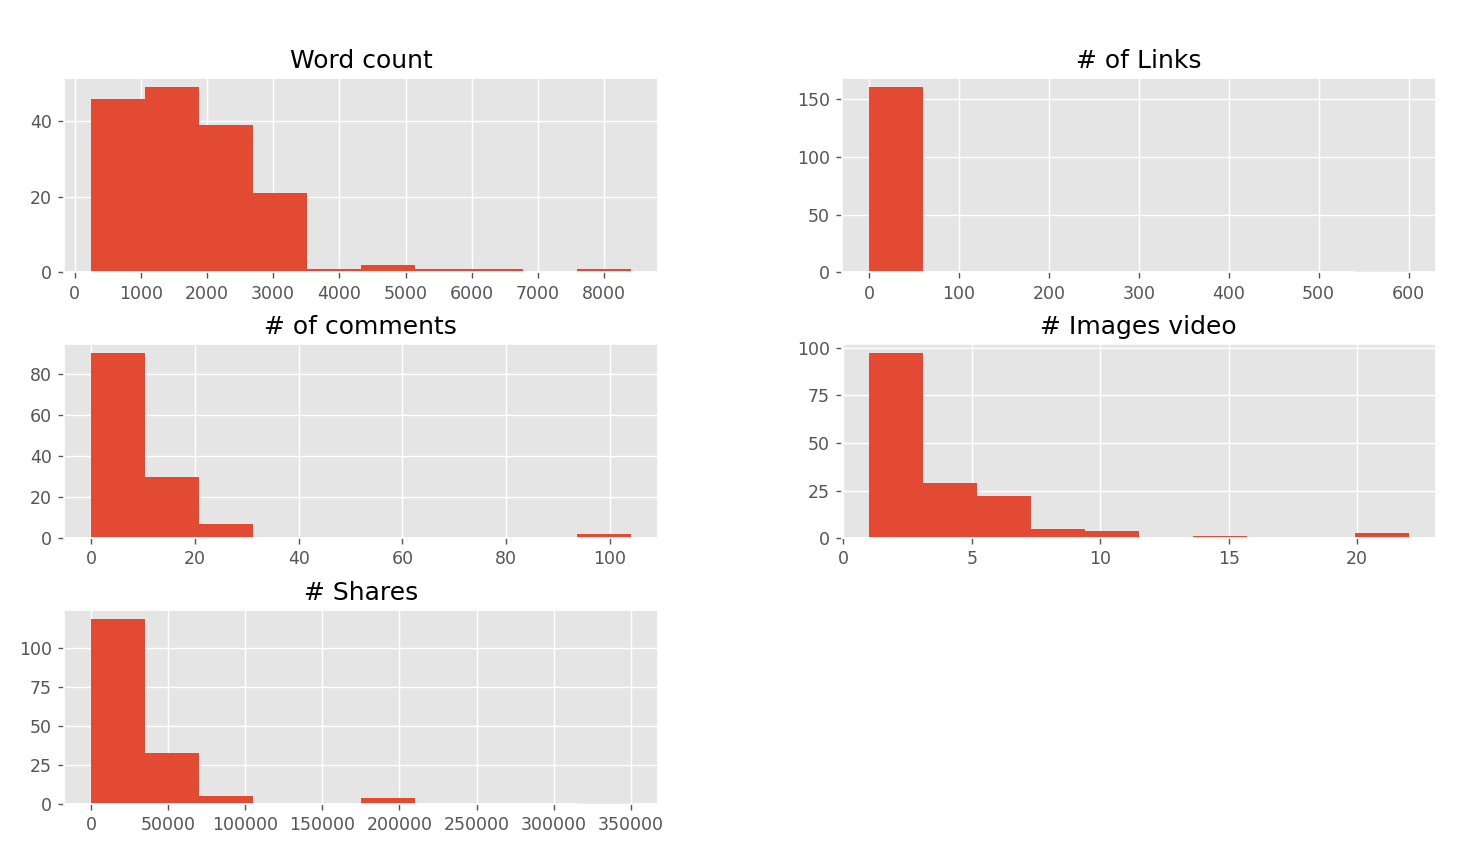
\includegraphics[width=0.9\linewidth]{img/a9_graficas.png}
    \caption{Histogramas del paso 2}
    \label{fig:figure2}
\end{figure}

\paragraph{}Gráfica de la relación entre el numero de palabras y el número de "shares" de un articulo:
\begin{figure}[H]
    \centering
    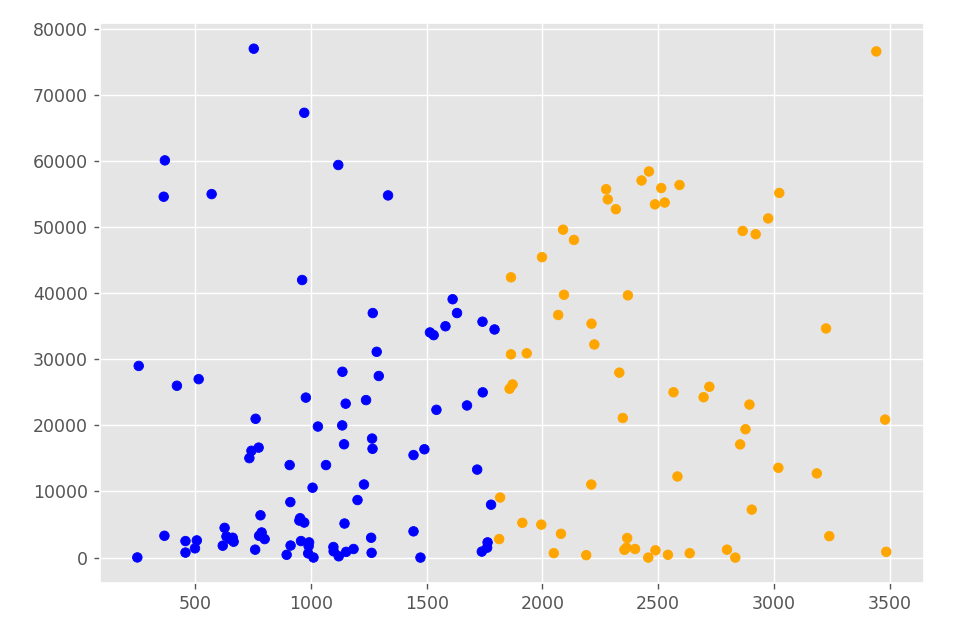
\includegraphics[width=0.5\linewidth]{img/a9_relacion.png}
    \caption{Gráfica de relación. Paso 3}
    \label{fig:figure2}
\end{figure}

Evaluación del modelo: De la ecuación de la recta $y=mX+b$ nuestra pendiente “m” es el coeficiente 5,69 y el término independiente “b” es 11200. El modelo regresa un error cuadrático muy grande y eso se ve reflejado en el puntaje de varianza que debería ser cercano a 1.0
\begin{figure}[H]
    \centering
    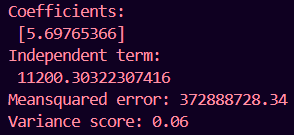
\includegraphics[width=0.4\linewidth]{img/a9_ecuacion.png}
    \caption{Paso 5}
    \label{fig:figure2}
\end{figure}

\paragraph{}Recta obtenida:
\begin{figure}[H]
    \centering
    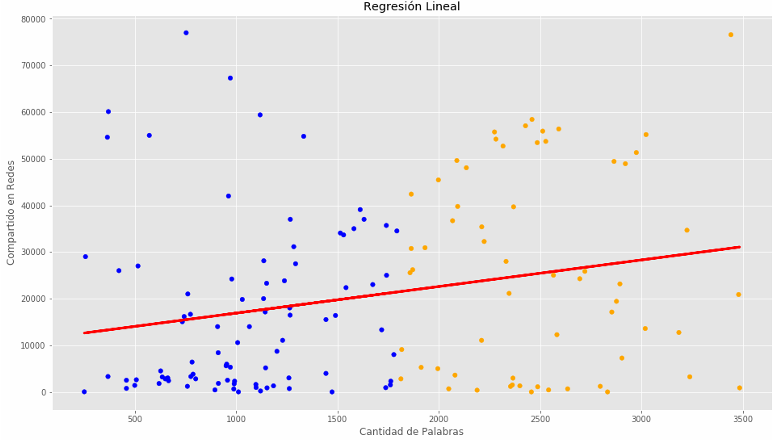
\includegraphics[width=0.8\linewidth]{img/a9_regresion.png}
    \caption{Paso 5}
    \label{fig:figure2}
\end{figure}

\paragraph{}Finalmente, la predicción para artículo de 2000 palabras es de 22,595 shares.\\

%--------------------------------------------------------------------
% Sección 4: Conclusión: Resume tus hallazgos y cualquier información obtenida de la actividad
\section{Conclusión}
Este ejercicio me ayudó a entender cómo funciona la regresión lineal en Python, pero también me dejó claro que predecir los shares solo con el número de palabras no es suficiente. El modelo mostró que, aunque más palabras tienden a significar más shares, la relación es débil (R² = 0.06), lo que quiere decir que hay otros factores importantes que no estamos considerando.

%--------------------------------------------------------------------
% Fin del documento
\end{document}